\documentclass[10pt, a4paper, twoside, onecolumn]{article}
\usepackage[backend=biber, sorting=none]{biblatex}
\addbibresource{refs.bib}
\usepackage[utf8]{inputenc}
\usepackage[T1]{fontenc}
\usepackage[polish]{babel}
\usepackage{uarial}
\usepackage[top=2.5cm,bottom=2.5cm,inner=3.5cm,outer=2.5cm]{geometry}
\usepackage{fancyhdr}
\usepackage{indentfirst}
\usepackage{graphicx}
\usepackage{hyperref}
\usepackage{float}
\usepackage{multirow}
\usepackage{amsmath}
\usepackage{amssymb}
\usepackage{sectsty}
\usepackage{etoolbox}
\usepackage[font=small]{caption}
\usepackage{physics}
\usepackage[version=4]{mhchem}
\usepackage{gensymb}
\usepackage{mathrsfs}
\usepackage{xfrac}
\usepackage{array}

%\usepackage{titling}
\usepackage{anyfontsize}
\usepackage{blindtext}

\graphicspath{ {./} }
\setlength{\parindent}{1.25cm}
\setlength{\parskip}{12pt}

\pagestyle{fancy}
\fancyhf{}
\fancyfoot[C]{\fontfamily{ua1}\fontsize{9pt}{9pt}\selectfont\thepage}
\renewcommand{\headrulewidth}{0pt}
\renewcommand{\footrulewidth}{0pt}

\renewcommand{\familydefault}{ua1}
\renewcommand{\baselinestretch}{1.5}

\setcounter{page}{3}
\raggedbottom

\sectionfont{\noindent\fontsize{12}{15}\selectfont}
\subsectionfont{\noindent\fontsize{10}{15}\selectfont\textit}
\subsubsectionfont{\noindent\fontsize{10}{15}\selectfont\normalfont\textit}

\BeforeBeginEnvironment{tabular}{\small}

\numberwithin{equation}{section}

\newcommand{\dbar}{d\hspace*{-0.08em}\bar{}\hspace*{0.1em}}

%\newcolumntype{L}{>{\(}l<{\)}}
%\newcolumntype{C}{>{\(}c<{\)}}
%\newcolumntype{R}{>{\(}r<{\)}}

% Problemy:
% W spisie kropki przy section
% Odpowiednie przerwy miedzy akapitami
% Opisy tabel nad tabela
% Odpowiednie przerwy miedzy opisem a tabela/rysunkiem
% Byc moze problemy z numerowaniem tabel, ale chyba jest na razie dobrze
% Przesunąc przecinki przy równaniach

\begin{document}
	\section*{Streszczenie}
	\begin{center}
		\textbf{Strona 3}
	\end{center}
	Termodynamika równowagowe wymaga założenia pewnych wyidealizowanych założeń, na przykład jednorodność parametrów intensywnych, maksimum entropii w układach izolowanych, minimum energii swobodnej Helmholtza w układach izotermiczno-izochorycznych, mininum entalpii swobodnej Gibbsa w układach izotermiczno-izobarycznych \cite{pudlik}. Takie założenie nie zawsze są możliwe, przykładowo dla szybko zachodzących zmian jak w przypadku eksplozji, albo dla układów, w których interesuje nas nie tylko stan układu po osiągnięciu przez niego stanu równowagi, ale też jego zachowania podczas tej przemiany. \par
	W pracy zająłem się głównie reakcjami chemicznymi oscylacyjnymi, które są przykładem czasowej struktury dyssypatywnej. Struktur takich nie można rozpatrywać w ramach termodynamiki liniowej, ponieważ są one typowe jedynie dla stanów nierównowagowych. Pierwsze takie reakcje odkryto w pierwszej połowie XX w., jednak jednym z nich jest organizm żywy, który można rozpatrywać jako bardzo skomplikowany układ termodynamiczny, w którym zachodzą cykliczne zmiany, na przykład stężenie hormonów oraz bicie serca. Najważniejszą reakcją dla rozwoju teorii reakcji oscylacyjnych jest reakcja Biełousowa-Żabotyńskiego. \par
	W pracy udało się zasymulować reakcje oscylacyjne wykorzystując modele Lotki, Lotki-Volterry oraz bruskelatora. Przeprowadzono teoretyczną analizę stabilności w stanach stacjonarnych oraz sprawdzono jej prawdziwość przy użyciu symulacji. 
	\pagebreak
	
	\section*{Abstract}
	\begin{center}
		\textbf{Strona 4}
	\end{center}
	%\blindtext \par
	%\blindtext \par
	%\blindtext \par
	%\blindtext \par
	\pagebreak
	
	\section*{Spis treści}
	\begin{center}
		\textbf{Strona 5}
	\end{center}
	\tableofcontents
	\pagebreak
	
	\section*{Wykaz oznaczeń}
	\addcontentsline{toc}{section}{Wykaz oznaczeń}
	\setlength{\parindent}{0cm}
	\begin{table}[H]
	\begin{tabular}{@{} ll}
		\(T\) & Temperatura \\
		\(S\) & Entropia \\
		\(p\) & Ciśnienie \\
		\(V\) & Objętość \\
		\(A\) & Powinowactwo chemiczne \\
		\(\xi\) & Liczba postępu reakcji \\
		\(s\) & Entropia na jednostkę objętości \\
		\(\mathscr{S}\) & Entropia na mol \\
		\(U\) & Energia wewnętrzna \\
		\(H=U+pV\) & Entalpia \\
		\(F=U-TS\) & Energia swobodna \\
		\(G=H-TS\) & Entalpia swobodna \\
		\(u, h, f, g\) & Energia, Entalpia, Energia swobodna oraz Entalpia swobodna na jednostkę objętości \\
		\(\mathscr{U, H, F, G}\) & Energia, Entalpia, Energia swobodna oraz Entalpia swobodna na mol \\
		\(C_{p}, C_{V}\) & Pojemności cieplne (\(c_{p}, c_{V}\) ciepła własciwe) \\
		\(N\) & Liczba cząsteczek (cząstek) \\
		\(\mu\) & Potencjał chemiczny
	\end{tabular}
	\end{table}
	\setlength{\parindent}{1.25cm}
	\pagebreak
	
	\section{Wstęp}
	
	Oscylacyjne reakcje chemiczne są przykładem procesu samoorganizacji w układach z reakcją chemiczną. W trakcie przebiegu takiej reakcji możemy zaobserwować oscylacyjne zmiany stężenia niektórych reagentów pojawiających się w czasie jej przebiegu. Zwykle są to przejściowe związki chemiczne, które pojawiają się w mechanizmie reakcji pomiędzy substratami a produktami. Zjawisko takiej samoorganizacji obserwujemy tylko wówczas, gdy układ z reakcją chemiczną jest w stanie dalekim od stanu równowagi termodynamicznej. \par
	Te oscylacyjne zmiany stężenia niektórych reagentów w oscylacyjnej reakcji chemicznej mogą odbywać się jednocześnie i tak samo w całej objętości układu, wówczas mówimy o powstaniu czasowej struktury dyssypatywnej. Jeśli stężenia tych reagentów zmieniają się zarówno w czasie jak i przestrzeni, wówczas mówimy o czasowo-przestrzennych strukturach dyssypatywnych. W tym drugim przypadku zaobserwujemy falę stężenia reagenta, która będzie przemieszczać się poprzez cała objętość układu. W trzecim przypadku te zmiany stężeń dotyczą tylko objętości układu, wówczas mówimy o przestrzennej strukturze dyssypatywnej. Wraz z osiągnięciem równowagi termodynamicznej w układzie opisane struktury zanikają. 
	
	% Wkleić przypadki struktur
	
	Wyjaśnienie tych oscylacji z punktu widzenia termodynamiki wymaga wyjścia poza termodynamikę równowagową. Termodynamika równowagowa zajmuje się procesami, w których ignoruje się upływ czasu, a przemiana jest kwazistatyczna. Oznacza to, że każdy stan pośredni można traktować jako stan równowagi termodynamicznej. Model taki jest wystarczający do opisu większości procesów. Można więc powiedzieć, że termodynamikę równowagową interesuje stan początkowy oraz końcowy. \par
	Dopiero termodynamika nierównowagowa jest teorią, która obejmuje to, co dzieje się w trakcie rzeczywistych przemian i jest ona konieczna do opisu reakcji oscylacyjnych. Pierwsze przesłanki o istnieniu takowych sięgają końca XIX wieku. Były to reakcje w układach heterogenicznych, jak na przykład pierścienie Lieseganga lub oscylacje prądu płynącego przez ogniwo galwaniczne. Wyjaśnienie tych zjawisk wymagało, aby układ byl heterogeniczny i było w zgodzie z entropią Boltzmanna, według której spontaniczna organizacja jest niemożliwa. \cite{orlik}\par
	Pierwszy model teoretyczny został przedstawiony przez Alfreda Lotka \cite{lotka}. Przez długi czas uważano, że nie mogą one przedstawiać rzeczywistych reakcji, ponieważ łamią II Z.T. według Boltzmanna. Jednak w 1921r. pokazano w reakcji Bray'a-Liebhafky'ego, że reakcje oscylacyjne w układach homogenicznych są możliwę. Jest to reakcja rokładu nadtlenku wodoru katalizowana jodanem (V). Jeszcze większy wpływ na rozwój termodynamiki nierównowagowej w kinetyce chemicznej były reakcje Biełousowa-Żabotyńskiego. Pierwszą reakcją z tej grupy została zaobserwowanaw 1959 w mieszaninie bromianu (V) potasu, siarczanie (VI) ceru (IV), kwasu malonowego oraz kwasu cytrynowego w rozcieńczonym kwasie siarkowym (VI). Została ona odkryta jako nieorganiczny analog cyklu Krebsa \cite{belousov_hist}. \par
	Innym zjawiskiem wyjaśnionym dzięki rozwoju termodynamiki nierównowagowej jest życie i ewolucja. Niepoprawne użycie II Z.T. może doprowadzić do wniosku, że powstanie złożonej struktury z chaosu powinno być niemożliwe. Wyjaśnienie takie błędnie wykorzystuje to prawo ignorując fakt, że układy biologiczne jak i cała Ziemia nie są układami izolowanymi. 
	
	\subsection{Generacja entropii}
	Wszystkie procesy rzeczywiste podlegają drugiej zasadzie termodynamiki, która określa różniczkową zmianę entropii \(\dd{S}\), w danych procesie nierównością
	\begin{equation}\label{II_Zasada_Termodynamiki}
		\dd{S}>0
	\end{equation}
	W powyższym zapisie pod symbolem \(\dd{S}\) kryje się suma różniczkowych zmian entropii otoczenia \(\dd{S_{ot}}\) i układu \(\dd{S_{uk}}\)
	\begin{equation}
		\dd{S}=\dd{S_{uk}}+\dd{S_{ot}}
	\end{equation}.
	W przyapadku układów izolowanych \(\dd{S}=\dd{S_{uk}}\), 
	więc w układach izolowanych entropia zawsze rośnie, a zatem spontaniczne uporządkowanie stabilnych struktur nie jest możliwe. \par
	Druga zasada termodynamiki dana wzorem \eqref{II_Zasada_Termodynamiki} rozstrzyga czy dany proces jest możliwy. Aby dodać tej zasadzie ilościowy charakter wprowadza się pojęcie produkcji entropii. W przypadku układu zamkniętego, w którym przebiega proces rzeczywisty drugą zasadę termodynamiki zapiszemy następującą nierównością: 
	\begin{equation}\label{II_Zasada_Termodynamiki_uklad}
		\dd{S_{uk}}>\frac{\dbar Q}{T_{ot}}
	\end{equation},
	gdzie \(\dd{S_{uk}}\) to różniczkowa zmiana entropii układu, \(\dbar Q\) to elementarne ciepło dostarczone do układu ze źródła o temperaturze \(T_{ot}\). Jeśli wymiana \(\dbar Q\) odbywa się w temperaturze \(T\) to 
	\begin{equation}
		\dd{S_{uk}}>\frac{\dbar Q}{T}
	\end{equation}.
	Z równania \eqref{II_Zasada_Termodynamiki} lub \eqref{II_Zasada_Termodynamiki_uklad} wynika, że w układach izolowanych % dokonczyc
	
	Z nierówności \eqref{II_Zasada_Termodynamiki} lub \eqref{II_Zasada_Termodynamiki_uklad} wynika, że różnicową zmianę entropii układu \(\dd{s_{uk}}\) możemy przedstawić jako sumę dwóch wkładów:
	\begin{equation}
		\dd{S_{uk}}=\dd_{e}S+\dd_{i}S
	\end{equation},
	gdzie \(\dd_{e}S=\frac{\dbar Q}{T}\), stanowi wkład do \(\dd{S_{uk}}\) wynikający tylko z wymiany ciepła, \(\dd_{i}S\) jest równy:
	\begin{equation}
		\dd_{i}S=\dd{S_{uk}}-\frac{\dbar Q}{T}
	\end{equation}.
	Składnik \(\dd_{i}S\) nazywany jest produkcją entropii. Warto zaznaczyć, że dla układu izolowanego \(\dd_{e}S=0\), stąd \(\dd{S_{uk}}=\dd_{i}S\). Natomiast na podstawie nierówności \eqref{II_Zasada_Termodynamiki} lub \eqref{II_Zasada_Termodynamiki_uklad} wynika, że \(\dd_{i}S>0\) w przemianach samorzutnych. \par
	Rozpatrzmy teraz drugą zasadę termodynamiki z punktu widzenia układu i otoczenia, która przyjmuje postać:
	\begin{equation}\label{II_Zasada_Termodynamiki_uklad_i_otoczenie}
		\dd{S_{ot}}+\dd{S_{ot}}>0
	\end{equation}, 
	gdzie symbolem \(\dd{S_{ot}}\) oznaczono różniczkową zmianę entropii otoczenia. Do nierówności \eqref{II_Zasada_Termodynamiki_uklad_i_otoczenie} wykorzystamy pojęcia zmieny entropii wynikającej z wymiany ciepła pomiędzy układem i otoczeniem oraz produkcji entropii, która może pojawić się w układzie i otoczeniu. Z nierówności \eqref{II_Zasada_Termodynamiki_uklad_i_otoczenie} otrzymujemy:
	\begin{equation}\label{II_Zasada_Termodynamiki_uklad_i_otoczenie_rozpisane}
		\dd_{e}S_{uk}+\dd_{i}S_{uk}+\dd_{e}S_{ot}+\dd_{i}S_{ot}>0
	\end{equation}.
	Jeśli wymiana ciepła zachodzi w temperaturze \(T\) to wówczas: \(\dd_{e}S_{uk}=-\dd_{e}S_{ot}\), otrzymujemy z \eqref{II_Zasada_Termodynamiki_uklad_i_otoczenie_rozpisane} 
	\begin{equation}\label{}
		\dd_{i}S_{uk}+\dd_{i}S_{ot}>0
	\end{equation}.
	Warunek obejmuje przypadek, w którym produkcja entropii \(\dd_{i}S_{uk}\) zmaleje na tyle, że \(\dd_{i}S_{ot}\) skompensuje ten niedostatek. W innym przypadku \(\dd_{i}S_{ot}\) może na tyle zmaleć, że \(\dd_{i}S_{uk}\) będzie kompensować ten niedostatek. W termodynamice nierównowagowej dokonujemy dodatkowo założenia:
	\begin{equation*}
		\dd_{i}S_{uk}>0
	\end{equation*}
	oraz
	\begin{equation*}
		\dd_{i}S_{ot}>0
	\end{equation*}.
	Z punkty widzenia pojedynczej komórki, dla której pozostałe stanowią otoczenie, oznacza to, że produkcja entropii w jej wnętrzu ma być nieujemna i podobnie dla pozostałych. To oznacza dalej, że w każdym dowolnie małym obszarze układu, w którym zachodzą procesy samorzutne następuje związane z nimi tworzenie entropii. To stwierdzenie stanowi treść drugiej hipotezy termodynamiki nierównowagowej, nazywaną lokalnym sformuowaniem drugiej zasady termodynamiki. Lokalne sformuowanie drugiej zasady termodynamiki nie wyklucza takiego przypadku, w którym w jednym i tym samym miejscu zachodzi kilka procesów, z których niektóre zmniejszają entropię \((\dd_{i}S<0)\), pod warunkiem, że oprócz nich obecne są procesy produkujące entropię \((\dd_{i}S>0)\), które z naddatkiem zwiększa entropię w tym miejscu. 
	




	Zmianę entropii układu można zapisać jako wynikającą z przepływu ciepła oraz samorzutnej generacji entropii: 
	\begin{equation}
		dS_{uk}=d_{e}S+d_{i}S_{uk}
	\end{equation}
	Dla układu zamkniętego: \(d_{e}S=0\), stąd wykorzystując \eqref{entropia_izolowany}:
	\begin{equation}
		dS_{uk}=d_{i}S_{uk}
	\end{equation}
	gdzie
	\begin{description}
		\item[\(dS_{uk}\)] całkowita zmiana entropii układu
		\item[\(d_{e}S=\frac{\dbar Q}{T_{uk}}\)] zmiana wynikająca z przepływu ciepła
		\item[\(d_{i}S_{uk}\geq 0\)] zmiana wynikająca z produkcji entropii
	\end{description}
	Dla każdego układu produkcja entropii jest dodatnia. Wynika z tego argumentu także, że jest to prawdziłe dla każdego podukładu należącego do danego układu niezależnie od jego wielkości. Zasada ta ma więc charakter lokalny. 
	
	
	
	\subsection{Termodynamika liniowa i nieliniowa}
	W ogólności natężenie przepływów termodynamicznych jest dowolną funkcją bodźców termodynamicznych: 
	\[J=f\left(X\right)\]
	Rozwinięcie w szereg Taylora tej funkcji wokół \(X_{0}\) jest
	\begin{equation}\label{ogolne_natezenie}
		J_{i}=J_{i}^{eq}+\sum_{k=1}^{n}\left[\frac{\partial J_{i}}{\partial X_{k}}\left(X_{k}-X_{k}^{eq}\right)\right]+\sum_{k=1}^{n}\left[\frac{1}{2}\frac{\partial^{2} J_{i}}{\partial X_{k}^{2}}\left(X_{k}-X_{k}^{eq}\right)^{2}\right]+\ldots
	\end{equation} % dodac elementy mieszane
	gdzie:
	\begin{description}
		\item[\(J\), \(J^{eq}\)] natężenie przepływów termodynamicznych oraz to natężenie w stanie równowagi
		\item[\(X\), \(X^{eq}\)] bodziec termodynamiczny i bodziec w stanie równowagi
	\end{description}
	Wiadomo, że \(J_{i}^{eq}=0\) oraz \(X_{k}^{eq}=0\), ponieważ jest to stan równowagi. \par
	W stanach zbliżonych do stanu równowagi można ograniczyć równanie \eqref{ogolne_natezenie} do następującego: 
	\begin{equation}\label{natezenie_liniowe}
		J_{i}=\sum_{k=1}^{n}\left[\frac{\partial J_{i}}{\partial X_{k}}X_{k}\right]
	\end{equation}
	Zapiszmy \(\frac{\partial J_{i}}{\partial X_{k}}\) jako \(L_{ik}\)
	\begin{equation}
		J_{i}=\sum_{k=1}^{n}L_{ik}X_{k}
	\end{equation}
	Natężenie przepływu może zależeć tylko od bodźca sprzężonego jak w prawie Fouriera \(\left(\boldsymbol{J}_{q}=-k\nabla T\right)\), Ficka \(\left(\boldsymbol{J}_{C}=-D\nabla C\right)\), są to wtedy procesy proste \cite{orlik}. Mogą one też zależeć od innych bodźców, przykładowo efekt Seebecka oraz Peltiera:
	\begin{gather}
		\boldsymbol{Q}=L_{qq}\Delta T+L_{qI}\Delta \phi \\
		\boldsymbol{I}=L_{Iq}\Delta T+L_{II}\Delta \phi
	\end{gather}\cite{Ceynowa2008}
	Występują w nich procesy krzyżowe; różnica temperatury wywołuje przepływ prądu oraz różnica potencjału elektrycznego wywołuje przepływ ciepła.
	Okazuje się, że współczynniki krzyżowe są sobie równe: \(L_{qI}=L_{Iq}\). Jest to reguła przemienności Onsagera, która została udowodniona doświadczalnie oraz na podstawie fizyki statystycznej. 
	% produkcja entropii
	Jednak w chemii termodynamika liniowa nie opisuje dobrze szybkości zachodzenia reakcji chemicznych, których prędkość zazwyczaj zależy od wyższych potęg stężenia związków. \par
	
	Termodynamika liniowa ma zastosowanie w większości przypadków technicznych, jednak nie są one w stanie opisać reakcji chemicznych, których szybkość zależy od wyższych niż 1 potęg stężenia składników. \par
	Istnieje kilka podejść w próbie wyjścia poza zakres liniowej termodynamiki nierównowagowej. Jedno z nich zakłada, że współczynniki \(L_{ij}\) zależą od bodźców i przepływów, a więc
	\begin{align}
		& \pdv{L_{ij}}{X_{k}}\neq 0, && \pdv{L_{ij}}{J_{k}}\neq 0
	\end{align}. 
	Równanie 
	% "f..."?
	zostaje zachowane, ale ten zabieg powoduje, że teoria staje się nieliniowa. \par
	Kolejne podejscie zakłada, że w rozwinięciu \eqref{ogolne_natezenie} uwzględnia większą liczbę wyrazów, przy zachowaniu niezależności współczynników rozwinięcia. Postuluje się jednocześnie, aby spełnione były relacje przemienności:
	\begin{align}
		L_{ij} &= L_{ji} \\
		L_{ijk} &= L_{jki} = L_{kij}
	\end{align}
	Jednak próby nie były owocne, a przemienność współczynników \(L_{ij}, L_{ijk}, \ldots\) trudna do uzależnienia. \par
	Bardziej owocne podejście do problemu wyjścia poza liniową termodynamikę nierównowagową, głównie w kontekście oscylacyjnych reakcji chemicznych, polegało na wykorzyskiwaniu metod stosowanych z teorii układów dynamicznych. Autorzy tej koncepcji pozostawiają postulat o istnieniu równowagi lokalnej. Hipoteza ta zakłada, że cały układ możemy podzielić na mniejsze podukłady (zwane niekiedy komórkami), w których parametry termodynamiczne są ściśle zdefiniowane, tak jak to mamy w zagadnieniach równowagowych. Parametry te w innych komórkach, mogą mieć inne wartości. \par
	Zakłada się tutaj, że te komórki są na tyle małe, iż możemy przyjąć, że parametry zmieniają się w sposób ciągły. Jednak z drugiej strony trzeba przyjąć, iż nie mogą one mieć bardzo małych rozmiarów. Ich makroskopowy charakter musi być zachowany przy założeniu dodatkowym, iż w każdej z nich panuje stan wewnętrznej równowagi. 
	
	
	
	
	
	
	Po zaprzestaniu wymuszania nierównowagi układ dąży do stanu równowagi z minimalną zerową produkcją entropii. Przy utrzymaniu stałego bodźca termodynamicznego układ dąży do stanu stacjonarnego o minimalnej dodatniej produkcji entropii. \par
	Rozwijając entropię \(s\left(E\right)\) po zakłóceniu \(\delta E\)w szereg Taylora otrzymujemy:
	\begin{equation}
		S=S^\circ+\left(\frac{\partial S}{\partial E}\right)^\circ \delta E+\frac{1}{2}\left(\frac{\partial^{2}S}{\partial E^{2}}\right)^\circ \left(\delta E\right)^2 + \ldots
	\end{equation}
	W stanie równowagi \(\left(\frac{\partial S}{\partial E}\right)^\circ=0\). Ograniczając szereg do wyrazu drugiego rzędu mamy:
	\begin{equation}
		S=S^\circ+\frac{1}{2}\left(\frac{\partial^{2}S}{\partial E^{2}}\right)^\circ \left(\delta E\right)^2=S^\circ+\frac{1}{2} \delta E\left(\frac{\partial \delta S}{\partial E}\right)^\circ=S^\circ+\frac{1}{2}\delta^{2}S
	\end{equation}
	Ze względu na maksimum entropii w stanie równowagi: \(\left(\delta^2 S\right)^\circ<0\)
	Można powiązać tą zależność z generacją entropii: 
	\begin{equation}
		\frac{\partial}{\partial t}\left(S-S^\circ\right)=\frac{1}{2}\frac{\partial}{\partial t}\delta^2 S=\sum_{i=1}^{n}J_{i}X_{i}=\sigma\geq0
	\end{equation}
	\subsection{Szybkość reakcji}
	
	Reakcje chemiczne można podzielić na dwie kategorie. Są to reakcje homogeniczne, czyli takie zachodzące w jednej fazie, oraz reakcje heterogeniczne, czyli między związkami w różnych fazach i zachodzące na granicy między nimi. Szybkość reakcji heterogenicznych jest trudniejsza do opisania, ponieważ zależy od szybkości dyfuzji, powierzchni rozdzielenia i innych czynników. %do uzupelnienia
	Szybkość reakcji homogenicznej w stałej temperaturze jest funkcją stężeń reagentów. Można ją wyrazić dla stałej objętości jako: 
	\begin{equation}
		v=\frac{1}{\nu_i}\dv{c_i}{t}
	\end{equation}
	Jest to wielkość niezależna od konkretnego reagenta. Można tak zdefiniowaną szybkość reakcji powiązać z szybkością zmiany liczby postępu reakcji:
	\begin{gather}
		v=\frac{1}{\nu_{i}}\dv{c_{i}}{t} \\
		\dd{c_{i}}=\frac{\dd{n_{i}}}{V} \\
		\dd{n_{i}}=\nu_{i}\dd{\xi} \\
		v=\frac{1}{V}\dv{\xi}{t}
	\end{gather}
	Dla reacji chemicznej w postaci ogólnej
	\begin{equation*}
		x_{1}X_{1}+x_{2}X_{2}+\ldots \rightarrow y_{1}Y_{1}+y_{2}Y_{2}+\ldots
	\end{equation*}
	szybkość ta ma ogólną postać:
	\begin{equation*}
		v=f\left(x_{1}, x_{2}, \ldots, y_{1}, y_{2}, \ldots\right)
	\end{equation*}
	Odpowiednie wzory są wyznaczane empirycznie i znacząca część z nich okazuje się mieć prostszą formę tej zależności:
	\begin{equation}\label{szybkosc reakcji}
		v=k x_{1}^{\alpha_1}x_{2}^{\alpha_2}\ldots y_{1}^{\beta_1}y_{2}^{\beta_2}\ldots
	\end{equation}
	Przykładowe reakcje i ich szybkości reakcji:
	\begin{align*}
		&\ce{2N2O2 -> 4NO2 + O2} &&v=k\left[\ce{N2O2}\right] \\
		&\ce{CH3COCH3 + I2 -> CH3COCH2I + HI} &&v=k\left[\ce{CH3COCH3}\right] \\
		&\ce{H2 + Br2 -> 2HBr} &&v=\frac{k_{1}\left[\ce{H2}\right]\left[\ce{Br2}\right]^{\sfrac{1}{2}}}{1+k_{2}\sfrac{\left[\ce{HBr}\right]}{\left[\ce{Br2}\right]}}
	\end{align*}
	Każdą z tych reakcji można rozdzielić na szereg występujących jednocześnie reakcji elementarnych. Przykładowo dla syntezy bromowodoru z cząsteczkowego wodoru i bromu:
	\begin{align*}
		&\ce{H2 + Br2 -> 2HBr} &&\text{reakcja sumaryczna} \\
		&\ce{Br2 -> 2Br^{.}} &&\text{reakcja elementarna} \\
		&\ce{Br^{.} + H2 -> HBr + H^{.}} &&\text{reakcja elementarna} \\
		&\ce{H^{.} + Br2 -> HBr + Br^{.}} &&\text{reakcja elementarna}
	\end{align*}
	Jednak analogiczna reakcja syntezy jodowodoru przebiega w sposób bezpośredni: 
	\begin{align*}
		&\ce{H2 + I2 -> 2HI}
	\end{align*}
	co oznacza, że każdą reakcję należy rozpatrywać osobno i nie ma jednego uniwersalnego schematu. \cite{pigon1}
	
	\subsection{Kataliza i autokataliza}
	Według równania \eqref{szybkosc reakcji} szybkość reakcji można zmienić przez zmianę stężenia reagentów lub zmianę stałej szybkości reakcji. Katalizatorami nazywamy związki zwiększające tą stała, natomiast związki zmniejszające katalizatorem ujemnym lub inhibitorem. Nie występują one w reakcji sumarycznej, ale występują w reakcjach elementarnych. Podobnie jak reakcje możemy podzielić katalizę na homogeniczną (zachodzącej w jednej fazie) oraz heterogeniczną (zachodząca na granicy faz). Szczególnym rodzajem reakcji katalitycznych jest autokataliza, w której produkt reakcji jest jednocześnie katalizatorem. Przykładem takiej reakcji jest hydroliza estrów w środowisku kwasowym: \cite{pigon1}
	\begin{center}
		\ce{RCOOC2H5 + 2H2O ->[H3O+] RCOO- + C2H5OH + H3O+}
	\end{center}
	
	\section{praca wlasna}
	\subsection{modele}
	\subsubsection{lotka}
	\begin{center}
		\ce{A ->[k_1] X} \\
		\ce{X + Y ->[k_2] 2Y} \\
		\ce{Y ->[k_3] produkty}
	\end{center}
	\begin{gather}
		\dv{[X]}{t}=k_{1}[A]-k_{2}[X][Y] \\
		\dv{[Y]}{t}=k_{2}[X][Y]-k_{3}[Y]
	\end{gather}
	\subsubsection{lotka-volterra}
	\begin{center}
		\ce{A + X ->[k_1] 2X} \\
		\ce{X + Y ->[k_2] 2Y} \\
		\ce{Y ->[k_3] produkty}
	\end{center}
	\begin{gather}
		\dv{[X]}{t}=k_{1}[A][X]-k_{2}[X][Y] \\
		\dv{[Y]}{t}=k_{2}[X][Y]-k_{3}[Y]
	\end{gather}
	\subsubsection{bruskelator}
	\begin{center}
		\ce{A ->[k_1] X} \\
		\ce{2X + Y ->[k_2] 3X} \\
		\ce{B + X ->[k_3] D + Y} \\
		\ce{X ->[k_4] E}
	\end{center}
	\begin{gather}
		\dv{[X]}{t}=k_{1}[A]+k_{2}[X]^{2}[Y]-k_{3}[B][X]-k_{4}[X] \\
		\dv{[Y]}{t}=-k_{2}[X]^{2}[Y]+k_{3}[B][X]
	\end{gather}
	\subsection{stabilnosc rozwiazan}
	Na potrzeby analizy można zredukować ilość parametrów danych równań różniczkowych stosując odpowiednie podstawienia. Najpierw należy wyznaczyć współrzędne punktu stacjonarnego. Analiza zostanie przedstawiona na przykładzie modelu Lotki, ale analogiczne wyprowadzenie można przeprowadzić dla każdego z tych modeli. W stanie stacjonarnym \(\dv{[X]}{t}=\dv{[Y]}{t}=0\)
	\begin{gather}
		k_{1}[A]-k_{2}[X]_{st}[Y]_{st}=0 \\
		k_{2}[X]_{st}[Y]_{st}-k_{3}[Y]_{st}=0
	\end{gather}
	Rozwiązując ten układ równań otrzymujemy
	\begin{gather}
		[X]_{st}=\frac{k_{3}}{k_{2}} \\
		[Y]_{st}=\frac{k_{1}[A]}{k_{3}}
	\end{gather}
	Wprowadzamy podstawienie
	\begin{align*}
		& x=\frac{[X]}{[X]_{st}} && y=\frac{[Y]}{[Y]_{st}} && \tau=k_{3}t && a=\frac{k_{1}k_{2}[A]}{k_{3}^{2}}
	\end{align*}
	i otrzymujemy po przekształceniach dla modelu Lotki:
	\begin{gather}
		\dv{x}{\tau}=a-axy \\
		\dv{y}{\tau}=xy-y
	\end{gather}
	Analogicznie dla modelu Lotki-Volterry:
	\begin{gather}
		\dv{x}{\tau}=ax-axy \\
		\dv{y}{\tau}=xy-y
	\end{gather}
	oraz modelu brusselator:
	\begin{gather}
		\dv{x}{\tau}=1+ax^{2}y-ax-x \\
		\dv{y}{\tau}=-bx^{2}y+bx
	\end{gather}
	Tak przygotowane równania mają stan stacjonarny w \(x=y=1\), co wynika z definicji. Zostaną one wykorzystane do numerycznego rozwiązania równań, ale na potrzeby analizy wprowadzam podstawienie
	\begin{align*}
		& \gamma=x-1 && \vartheta=y-1
	\end{align*}
	Co przesuwa stan stacjonarny do \(\gamma=\vartheta=0\). Otrzymujemy dla modelu Lotki:
	\begin{gather}
		\dv{\gamma}{\tau}=-a\gamma\vartheta-a\gamma-a\vartheta \\
		\dv{\vartheta}{\tau}=\gamma\vartheta+\gamma
	\end{gather}
	Dla modelu Lotki-Volterry:
	\begin{gather}
		\dv{\gamma}{\tau}=-a\gamma\vartheta-a\vartheta \\
		\dv{\vartheta}{\tau}=\gamma\vartheta+\gamma
	\end{gather}
	Dla modelu brusselator:
	\begin{gather}
		\dv{\gamma}{\tau}=a\gamma^{2}\vartheta+a\gamma^{2}+2a\gamma\vartheta+a\gamma+a\vartheta-\gamma \\
		\dv{\vartheta}{\tau}=-b\gamma^{2}\vartheta-b\gamma^{2}-2b\gamma\vartheta-b\gamma-b\vartheta
	\end{gather}
	Istnienie punktu stacjonarnego nie oznacza, że jest on atraktorem. Badanie charakteru punktu stacjonarnego układu równań rózniczkowych nieliniowych jest trudne, ale można wprowadzić pewne uproszczenie i zlinearyzować ten układ. Oznacza to rozwiniecie funcji po prawej stronie równań w szereg Taylora i ograniczenie go do elementu liniowego. Działanie to jest uzasadnione tym, że badamy jedynie najbliższe otoczenie i kolejne składniki mają mniejszy wkład im bliżej punktu stacjonarnego. \par
	Po linearyzacji otrzymujemy dla modelu Lotki:
	\begin{gather}
		\dv{\gamma}{\tau}=-a\gamma-a\vartheta \\
		\dv{\vartheta}{\tau}=\gamma
	\end{gather}
	Dla modelu Lotki-Volterry:
	\begin{gather}
		\dv{\gamma}{\tau}=-a\vartheta \\
		\dv{\vartheta}{\tau}=\gamma
	\end{gather}
	Dla modelu brusselator:
	\begin{gather}
		\dv{\gamma}{\tau}=(a-1)\gamma+a\vartheta \\
		\dv{\vartheta}{\tau}=-b\gamma-b\vartheta
	\end{gather}
	Można teraz badać stany stabilne metodami równań różniczkowych liniowych. Stabilność zależy od wartości własnych macierzy stałych. Dla modelu Lotki:
	\begin{gather}
		\det
		\begin{pmatrix}
			-a-\lambda & -a \\
			1 & -\lambda
		\end{pmatrix}
		=\lambda^{2}+a\lambda+a=0 \\
		\lambda_{1}+\lambda_{2}=-a \\
		\lambda_{1}\lambda_{2}=a
	\end{gather}
	Dla modelu Lotki-Volterry:
	\begin{gather}
		\det
		\begin{pmatrix}
			-\lambda & -a \\
			1 & -\lambda
		\end{pmatrix}
		=\lambda^{2}+a=0 \\
		\lambda_{1}+\lambda_{2}=0 \\
		\lambda_{1}\lambda_{2}=a
	\end{gather}
	Dla modelu brusselator:
	\begin{gather}
		\det
		\begin{pmatrix}
			a-1-\lambda & a \\
			-b & -b-\lambda
		\end{pmatrix}
		=\lambda^{2}+(-a+b+1)\lambda+b=0 \\
		\lambda_{1}+\lambda_{2}=a-b-1 \\
		\lambda_{1}\lambda_{2}=b
	\end{gather}
	\begin{table}[H]
		\centering
		\begin{tabular}{|c|c|c|c|}\cline{1-4}
			& \(\lambda_{1}+\lambda_{2}<0\) & \(\lambda_{1}+\lambda_{2}=0\) & \(\lambda_{1}+\lambda_{2}>0\) \\ \cline{1-4}
			\(\left(\frac{\lambda_{1}+\lambda_{2}}{2}\right)^{2}<\lambda_{1}\lambda_{2}\) & 
			\begin{tabular}{c} %11
				\(\lambda_{1}, \lambda_{2}\in\mathbb{C}\) \\
				\(\Re{\lambda_{1}}=\Re{\lambda_{2}}<0\) \\
				\(\lambda_{1}=\overline{\lambda_{2}}\) 
			\end{tabular}
			& \multirow{2}{*}{
			\begin{tabular}{c} %(1-2)2
				\(\lambda_{1}, \lambda_{2}\in\mathbb{C}\) \\
				\(\Re{\lambda_{1}}=\Re{\lambda_{2}}=0\) \\
				\(\lambda_{1}=-\lambda_{2}\) 
			\end{tabular}
			} & 
			\begin{tabular}{c} %13
				\(\lambda_{1}, \lambda_{2}\in\mathbb{C}\) \\
				\(\Re{\lambda_{1}}=\Re{\lambda_{2}}>0\) \\
				\(\lambda_{1}=\overline{\lambda_{2}}\) 
			\end{tabular} 
			\\ \cline{1-2}\cline{4-4}
			\(0<\lambda_{1}\lambda_{2}\leq\left(\frac{\lambda_{1}+\lambda_{2}}{2}\right)^{2}\) & 
			\begin{tabular}{c} %21
				\(\lambda_{1}, \lambda_{2}\in\mathbb{R}\) \\
				\(\lambda_{1}, \lambda_{2}<0\) 
			\end{tabular}
			& &
			\begin{tabular}{c} %23
				\(\lambda_{1}, \lambda_{2}\in\mathbb{R}\) \\
				\(\lambda_{1}, \lambda_{2}>0\) 
			\end{tabular}
			\\ \cline{1-4}
			\(\lambda_{1}\lambda_{2}=0\) & 
			\begin{tabular}{c} %31
				\(\lambda_{1}, \lambda_{2}\in\mathbb{R}\) \\
				\(\lambda_{1}<\lambda_{2}=0\) 
			\end{tabular}
			& 
			\begin{tabular}{c} %32
				\(\lambda_{1}, \lambda_{2}\in\mathbb{R}\) \\
				\(\lambda_{1}=\lambda_{2}=0\) 
			\end{tabular}
			& 
			\begin{tabular}{c} %33
				\(\lambda_{1}, \lambda_{2}\in\mathbb{R}\) \\
				\(0=\lambda_{1}<\lambda_{2}\) 
			\end{tabular}
			\\ \cline{1-4}
			\(\lambda_{1}\lambda_{2}<0\) & 
			\begin{tabular}{c} %41
				\(\lambda_{1}, \lambda_{2}\in\mathbb{R}\) \\
				\(0<\lambda_{2}<-\lambda_{1}\) 
			\end{tabular}
			& 
			\begin{tabular}{c} %42
				\(\lambda_{1}, \lambda_{2}\in\mathbb{R}\) \\
				\(0<\lambda_{2}=-\lambda_{1}\) 
			\end{tabular}
			&
			\begin{tabular}{c} %43
				\(\lambda_{1}, \lambda_{2}\in\mathbb{R}\) \\
				\(0>\lambda_{1}>-\lambda_{2}\) 
			\end{tabular}
			\\ \cline{1-4}
		\end{tabular}
		\caption{Warunki stabilności}
	\end{table}
	
	\begin{table}[H]
		\centering
		\begin{tabular}{|c|c|c|c|}\cline{1-4}
			& \(\lambda_{1}+\lambda_{2}<0\) & \(\lambda_{1}+\lambda_{2}=0\) & \(\lambda_{1}+\lambda_{2}>0\) \\ \cline{1-4}
			\(\left(\frac{\lambda_{1}+\lambda_{2}}{2}\right)^{2}<\lambda_{1}\lambda_{2}\) & 
			\begin{tabular}{c} %11
				\(0<a<4\)
			\end{tabular}
			& \multirow{2}{*}{
				\begin{tabular}{c} %(1-2)2
					-
				\end{tabular}
			} & 
			\begin{tabular}{c} %13
				-
			\end{tabular} 
			\\ \cline{1-2}\cline{4-4}
			\(0<\lambda_{1}\lambda_{2}\leq\left(\frac{\lambda_{1}+\lambda_{2}}{2}\right)^{2}\) & 
			\begin{tabular}{c} %21
				\(4\leq a\)
			\end{tabular}
			& &
			\begin{tabular}{c} %23
				-
			\end{tabular}
			\\ \cline{1-4}
			\(\lambda_{1}\lambda_{2}=0\) & 
			\begin{tabular}{c} %31
				-
			\end{tabular}
			& 
			\begin{tabular}{c} %32
				\(a=0\)
			\end{tabular}
			& 
			\begin{tabular}{c} %33
				-
			\end{tabular}
			\\ \cline{1-4}
			\(\lambda_{1}\lambda_{2}<0\) & 
			\begin{tabular}{c} %41
				-
			\end{tabular}
			& 
			\begin{tabular}{c} %42
				-
			\end{tabular}
			&
			\begin{tabular}{c} %43
				\(a<0\)
			\end{tabular}
			\\ \cline{1-4}
		\end{tabular}
		\caption{Warunki dla modelu Lotki}
	\end{table}

	\begin{table}[H]
		\centering
		\begin{tabular}{|c|c|c|c|}\cline{1-4}
			& \(\lambda_{1}+\lambda_{2}<0\) & \(\lambda_{1}+\lambda_{2}=0\) & \(\lambda_{1}+\lambda_{2}>0\) \\ \cline{1-4}
			\(\left(\frac{\lambda_{1}+\lambda_{2}}{2}\right)^{2}<\lambda_{1}\lambda_{2}\) & 
			\begin{tabular}{c} %11
				-
			\end{tabular}
			& \multirow{2}{*}{
				\begin{tabular}{c} %(1-2)2
					\(0<a\)
				\end{tabular}
			} & 
			\begin{tabular}{c} %13
				-
			\end{tabular} 
			\\ \cline{1-2}\cline{4-4}
			\(0<\lambda_{1}\lambda_{2}\leq\left(\frac{\lambda_{1}+\lambda_{2}}{2}\right)^{2}\) & 
			\begin{tabular}{c} %21
				-
			\end{tabular}
			& &
			\begin{tabular}{c} %23
				-
			\end{tabular}
			\\ \cline{1-4}
			\(\lambda_{1}\lambda_{2}=0\) & 
			\begin{tabular}{c} %31
				-
			\end{tabular}
			& 
			\begin{tabular}{c} %32
				\(a=0\) 
			\end{tabular}
			& 
			\begin{tabular}{c} %33
				-
			\end{tabular}
			\\ \cline{1-4}
			\(\lambda_{1}\lambda_{2}<0\) & 
			\begin{tabular}{c} %41
				-
			\end{tabular}
			& 
			\begin{tabular}{c} %42
				\(a<0\)
			\end{tabular}
			&
			\begin{tabular}{c} %43
				-
			\end{tabular}
			\\ \cline{1-4}
		\end{tabular}
		\caption{Warunki dla modelu Lotki-Volterry}
	\end{table}

	\begin{table}[H]
		\centering
		\begin{tabular}{|c|c|c|c|}\cline{1-4}
			& \(\lambda_{1}+\lambda_{2}<0\) & \(\lambda_{1}+\lambda_{2}=0\) & \(\lambda_{1}+\lambda_{2}>0\) \\ \cline{1-4}
			\(\left(\frac{\lambda_{1}+\lambda_{2}}{2}\right)^{2}<\lambda_{1}\lambda_{2}\) & 
			\begin{tabular}{c} %11
				\(b+1-2\sqrt{b}<a<b+1\) \\
				\(0<b\)
			\end{tabular}
			& \multirow{2}{*}{
				\begin{tabular}{c} %(1-2)2
					 \(a=b+1\) \\
					 \(0<b\)
				\end{tabular}
			} & 
			\begin{tabular}{c} %13
				\(b+1<a<b+1+2\sqrt{b}\) \\
				\(0<b\)
			\end{tabular} 
			\\ \cline{1-2}\cline{4-4}
			\(0<\lambda_{1}\lambda_{2}\leq\left(\frac{\lambda_{1}+\lambda_{2}}{2}\right)^{2}\) & 
			\begin{tabular}{c} %21
				\(a\leq b+1-2\sqrt{b}\) \\
				\(0<b\)
			\end{tabular}
			& &
			\begin{tabular}{c} %23
				\(b+1+2\sqrt{b}\leq a\) \\
				\(0<b\)
			\end{tabular}
			\\ \cline{1-4}
			\(\lambda_{1}\lambda_{2}=0\) & 
			\begin{tabular}{c} %31
				\(a<1\) \\
				\(b=0\)
			\end{tabular}
			& 
			\begin{tabular}{c} %32
				\(a=1\) \\
				\(b=0\) 
			\end{tabular}
			& 
			\begin{tabular}{c} %33
				\(1<a\) \\
				\(b=0\)
			\end{tabular}
			\\ \cline{1-4}
			\(\lambda_{1}\lambda_{2}<0\) & 
			\begin{tabular}{c} %41
				\(a<b+1\) \\
				\(b<0\)
			\end{tabular}
			& 
			\begin{tabular}{c} %42
				\(a=b+1\) \\
				\(b<0\)
			\end{tabular}
			&
			\begin{tabular}{c} %43
				\(b+1<a\) \\
				\(b<0\)
			\end{tabular}
			\\ \cline{1-4}
		\end{tabular}
		\caption{Warunki dla modelu brusselator}
	\end{table}
	\subsection{metody różniczkowe}
	Układ równań liniowych pierwszego rzędu o stałych współczynnikach ma w ogólności rozwiązanie analityczne \cite{palczewski}
	\begin{gather}
		\dv{X(t)}{t}=RX(t) \\
		X(t)=\exp(Rt)X(0)
	\end{gather}
	Rozpatrywane układy jednak nie mają rozwiązania analitycznego i należy je rozwiązać metodami numerycznymi. \par
	\begin{table}[H]\label{tab:schematy}
		\centering
		\begin{tabular}{|l|l|c|c|}
			\hline
			 & Wzór & \(p\) & \(A_{p+1}\) \\
			\hline
			1 & \(y_{n+1}=y_{n}+hy'_{n}\) & \(1\) & \(\frac{1}{2}\) \\
			\hline
			2 & \(y_{n+1}=y_{n}+\frac{h}{2}(3y'_{n}-y'_{n-1})\) & \(2\) & \(\frac{5}{12}\) \\
			\hline
			3 & \(y_{n+1}=y_{n}+\frac{h}{12}(23y'_{n}-16y'_{n-1}+5y'_{n-2})\) & \(3\) & \(\frac{3}{8}\) \\
			\hline
			4 & \(y_{n+1}=y_{n}+\frac{h}{24}(55y'_{n}-59y'_{n-1}+37y'_{n-2}-9y'_{n-3})\) & \(4\) & \(\frac{251}{720}\) \\
			\hline
			5 & \(y_{n+1}=y_{n-3}+\frac{4h}{3}(2y'_{n}-y'_{n-1}+2y'_{n-2})\) & \(4\) & \(\frac{14}{45}\) \\
			\hline
		\end{tabular}
		\caption{Schematy różnicowe}
	\end{table}
	gdzie \(h\) jest krokiem czasowym, \(p\) to najwyższa wykładnik potęgi \(h^{s}\), przy których współczynnik wynosi \(0\), a \(A_{p+1}\) jest współczynnikiem przy kolejnej potędze.
	\begin{figure}[H]\label{img:lotka}
		\centering
		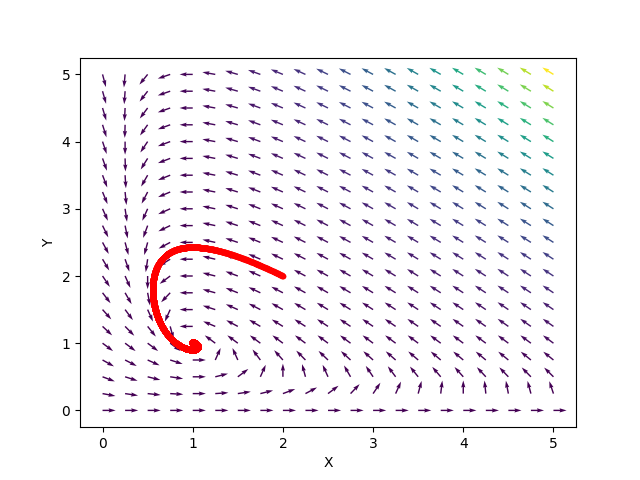
\includegraphics{lotka.png}
		\caption{Model Lotki; \(k_{1}=k_{2}=k_{3}=A=1\)}
	\end{figure}
	\begin{figure}[H]\label{img:lotka_volterra}
		\centering
		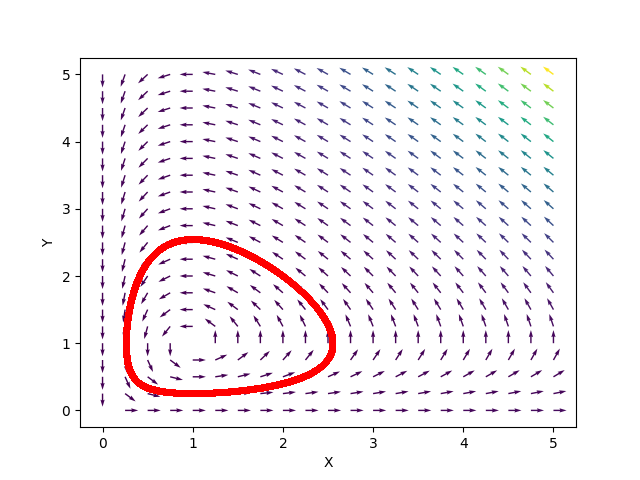
\includegraphics{lotka_volterra.png}
		\caption{Model Lotki-Volterry; \(k_{1}=k_{2}=k_{3}=A=1\)}
	\end{figure}
	\begin{figure}[H]\label{img:brusselator}
		\centering
		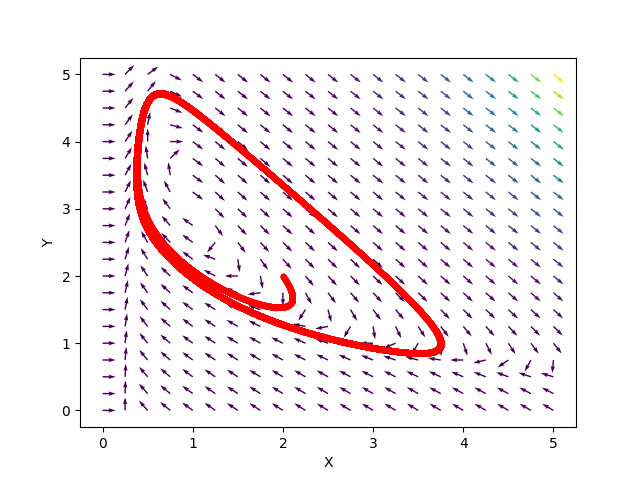
\includegraphics{brusselator.png}
		\caption{Model brusselator; \(k_{1}=k_{2}=k_{3}=k_{4}=A=1\)}
	\end{figure}
	%\blindtext
	\section{Sekcja 2}
	%\blindtext
	\section{Sekcja 3}
	%\blindtext
	\section{Sekcja 4}
	%\blindtext 
	\pagebreak
	%\section*{Wykaz literatury}
	\addcontentsline{toc}{section}{Wykaz literatury}
	\printbibliography[title=Wykaz literatury]
	\pagebreak
	\section*{Wykaz rysunków}
	\addcontentsline{toc}{section}{Wykaz rysunków}
	\pagebreak
	\section*{Wykaz tabel}
	\addcontentsline{toc}{section}{Wykaz tabel}
	\pagebreak
	\section*{Dodatek A}
	\addcontentsline{toc}{section}{Dodatek A}
	\begin{gather}
		\dd{u}=T\dd{s}-p\dd{V}+\sum_{i}\mu_{i}\dd{n_{i}}; \dd{V}=0 \label{dod A: 1} \\
		\dd{s}=\frac{1}{T}\dd{u}-\sum_{i}\frac{\mu_{i}}{T}\dd{n_{i}} \label{dod A: 2} \\
		\dv{s}{t}=\frac{1}{T}\dv{u}{t}-\sum_{i}\frac{\mu_{i}}{T}\dv{n_{i}}{t} \label{dod A: 3} \\
		\vb{J}_{s}=\frac{1}{T}\vb{J}_{u}-\sum_{i}\frac{\mu_{i}}{T}\vb{J}_{i} \label{dod A: 4}
	\end{gather}
	Równania ciągłości:
	\begin{gather}
		\dv{s}{t}=-\div{\vb{J}_{s}}+\sigma \label{dod A: 5} \\
		\dv{u}{t}=-\div{\vb{J}_{u}} \label{dod A: 6} \\
		\dv{n_{i}}{t}=-\div{\vb{J}_{i}}+\dv{n_{i;reak}}{t}; \dd{n_{i;reak}}=\sum_{r}\nu_{ir}\dd{\xi_{r}} \label{dod A: 7} \\
		\dv{n_{i}}{t}=-\div{\vb{J}_{i}}+\sum_{r}\nu_{ir}\dv{\xi_{r}}{t} \label{dod A: 8}
	\end{gather}
	Podstawiając \eqref{dod A: 4}, \eqref{dod A: 6} oraz \eqref{dod A: 8} do \eqref{dod A: 5} otrzymujemy: 
	\begin{equation} \label{dod A: 9}
		\dv{s}{t}=\frac{1}{T}\dv{u}{t}-\sum_{i}\frac{\mu_{i}}{T}\dv{n_{i}}{t}-\left[\vb{J}_{u}\vdot\grad{\frac{1}{T}}-\sum_{i}\vb{J}_{i}\cdot\grad{\frac{\mu_{i}}{T}}-\frac{1}{T}\sum_{r}\sum_{i}\nu_{ir}\mu_{i}\dv{\xi_{r}}{t}\right]+\sigma
	\end{equation}
	Wprowadzamy pojęcie powinowactwa chemicznego: 
	\begin{equation}
		A_{r}=-\sum_{i}\nu_{ir}\mu_{i} \\
	\end{equation}
	Równanie \eqref{dod A: 9} przybiera postać:
	\begin{equation}
		\dv{s}{t}=\frac{1}{T}\dv{u}{t}-\sum_{i}\frac{\mu_{i}}{T}\dv{n_{i}}{t}-\left[\vb{J}_{u}\vdot\grad{\left(\frac{1}{T}\right)}-\sum_{i}\vb{J}_{i}\cdot\grad{\left(\frac{\mu_{i}}{T}\right)}+\sum_{r}\frac{A_{r}}{T}\dv{\xi_{r}}{t}\right]+\sigma
	\end{equation}
	Otrzymujemy z porównania tego wzoru z \eqref{dod A: 3}:
	\begin{equation}
		\sigma=\vb{J}_{u}\vdot\grad{\left(\frac{1}{T}\right)}-\sum_{i}\vb{J}_{i}\cdot\grad{\left(\frac{\mu_{i}}{T}\right)}+\sum_{r}\frac{A_{r}}{T}\dv{\xi_{r}}{t}
	\end{equation}
	Z analogicznego wyprowadzenia dla entalpii i założenia stałego ciśnienia:
	\begin{equation}
		\sigma=\vb{J}_{h}\vdot\grad{\left(\frac{1}{T}\right)}-\sum_{i}\vb{J}_{i}\cdot\grad{\left(\frac{\mu_{i}}{T}\right)}+\sum_{r}\frac{A_{r}}{T}\dv{\xi_{r}}{t}
	\end{equation}
	\begin{table}[H]
	\centering
	\begin{tabular}{|l|c|c|}
		\hline
		Proces & Przepływ & Siła termodynamiczna \\
		\hline
		Transport energii & \(\vb{J}_u\) & \(\grad{\left(\frac{1}{T}\right)}\) \\
		Transport entalpii & \(\vb{J}_h\) & \(\grad{\left(\frac{1}{T}\right)}\) \\
		Dyfuzja & \(\vb{J}_i\) & \(-\grad{\left(\frac{\mu_{i}}{T}\right)}\) \\
		Reakcja chemiczna & \(J_{r}=\dv{\xi_{r}}{t}\) & \(\frac{A_r}{T}\) \\
		\hline
	\end{tabular}
	\end{table}
	\pagebreak
	\section{Dodatek B}
	\begin{gather}
		U=U\left(S, V, \xi\right) \\
		H=H\left(S, p, \xi\right) \\
		F=F\left(T, V, \xi\right) \\
		G=G\left(T, p, \xi\right)
	\end{gather}
	\begin{gather}
		\dd{U}=T\dd{S}-p\dd{V}-A\dd{\xi} \\
		\dd{H}=T\dd{S}+V\dd{p}-A\dd{\xi} \\
		\dd{F}=-S\dd{T}-p\dd{V}-A\dd{\xi} \\
		\dd{G}=-S\dd{T}+V\dd{p}-A\dd{\xi}
	\end{gather}
	Pochodne cząstkowe:
	\begin{table}[H]
	\centering
	\begin{tabular}{lll}
		\(\left(\pdv{U}{S}\right)_{V, \xi}=T\) & \(\left(\pdv{U}{V}\right)_{S, \xi}=-p\) & \(\left(\pdv{U}{\xi}\right)_{S, V}=-A\) \\
		\(\left(\pdv{H}{S}\right)_{p, \xi}=T\) & \(\left(\pdv{H}{p}\right)_{S, \xi}=V\) & \(\left(\pdv{H}{\xi}\right)_{S, p}=-A\) \\
		\(\left(\pdv{F}{T}\right)_{V, \xi}=-S\) & \(\left(\pdv{F}{V}\right)_{T, \xi}=-p\) & \(\left(\pdv{F}{\xi}\right)_{T, V}=-A\) \\
		\(\left(\pdv{G}{T}\right)_{p, \xi}=-S\) & \(\left(\pdv{G}{p}\right)_{T, \xi}=V\) & \(\left(\pdv{G}{\xi}\right)_{T, p}=-A\) \\
	\end{tabular}
	\end{table}
	U, H, F, G są funkcjami stanu, więc pochodne mieszane są sobie równe:
	\begin{table}[H]
	\centering
	\begin{tabular}{lll}
		\(\left(\pdv{T}{V}\right)_{S, \xi}=-\left(\pdv{p}{S}\right)_{V, \xi}\) & \(\left(\pdv{T}{\xi}\right)_{S, V}=-\left(\pdv{A}{S}\right)_{V, \xi}\) & \(\left(\pdv{p}{\xi}\right)_{S, V}=\left(\pdv{A}{V}\right)_{S, \xi}\) \\
		\(\left(\pdv{T}{p}\right)_{S, \xi}=\left(\pdv{V}{S}\right)_{p, \xi}\) & \(\left(\pdv{T}{\xi}\right)_{S, p}=-\left(\pdv{A}{S}\right)_{p, \xi}\) & \(\left(\pdv{V}{\xi}\right)_{S, p}=-\left(\pdv{A}{p}\right)_{S, \xi}\) \\
		\(\left(\pdv{S}{V}\right)_{T, \xi}=\left(\pdv{p}{T}\right)_{V, \xi}\) & \(\left(\pdv{S}{\xi}\right)_{T, V}=\left(\pdv{A}{T}\right)_{V, \xi}\) & \(\left(\pdv{p}{\xi}\right)_{T, V}=\left(\pdv{A}{V}\right)_{T, \xi}\) \\
		\(\left(\pdv{S}{p}\right)_{T, \xi}=-\left(\pdv{V}{T}\right)_{p, \xi}\) & \(\left(\pdv{S}{\xi}\right)_{T, p}=\left(\pdv{A}{T}\right)_{p, \xi}\) & \(\left(\pdv{V}{\xi}\right)_{T, p}=-\left(\pdv{A}{p}\right)_{T, \xi}\)
	\end{tabular}
	\end{table}
	Pochodne po temperaturze:
	\begin{table}[H]
	\centering
	\begin{tabular}{ll}
		\(\left(\pdv{U}{T}\right)_{V, \xi}=C_{V, \xi}\) & \(\left(\pdv{S}{T}\right)_{V, \xi}=\frac{C_{V, \xi}}{T}\) \\
		\(\left(\pdv{H}{T}\right)_{p, \xi}=C_{p, \xi}\) & \(\left(\pdv{S}{T}\right)_{p, \xi}=\frac{C_{p, \xi}}{T}\) \\
		\(\left(\pdv{F}{T}\right)_{V, \xi}=-S\) & \(\left(\pdv{A}{T}\right)_{V, \xi}=\Delta_{r}S_{V}\) \\
		\(\left(\pdv{G}{T}\right)_{p, \xi}=-S\) & \(\left(\pdv{A}{T}\right)_{p, \xi}=\Delta_{r}S_{p}\)
	\end{tabular}
	\end{table}
	\begin{gather}
		A\dd{\xi}=T\dd{S}-\dd{U}-p\dd{V} \\
		A\dd{\xi}=T\dd{S}-\dd{H}+V\dd{p}
	\end{gather}
	Podstawiając do tego odpowiednio: 
	\begin{gather}
	\begin{split}
		\dd{S}=\left(\pdv{S}{T}\right)_{V, \xi}\dd{T}+\left(\pdv{S}{V}\right)_{T, \xi}\dd{V}+\left(\pdv{S}{\xi}\right)_{T, V}\dd{\xi} \\
		\dd{U}=\left(\pdv{U}{T}\right)_{V, \xi}\dd{T}+\left(\pdv{U}{V}\right)_{T, \xi}\dd{V}+\left(\pdv{U}{\xi}\right)_{T, V}\dd{\xi}
	\end{split} \\
	\begin{split}
		\dd{S}=\left(\pdv{S}{T}\right)_{p, \xi}\dd{T}+\left(\pdv{S}{p}\right)_{T, \xi}\dd{p}+\left(\pdv{S}{\xi}\right)_{T, p}\dd{\xi} \\
		\dd{H}=\left(\pdv{H}{T}\right)_{p, \xi}\dd{T}+\left(\pdv{H}{p}\right)_{T, \xi}\dd{p}+\left(\pdv{H}{\xi}\right)_{T, p}\dd{\xi}
	\end{split}
	\end{gather}
	otrzymujemy:
	\begin{multline}
		A\dd{\xi}=\left[T\left(\dv{S}{T}\right)_{V, \xi}-\left(\pdv{U}{T}\right)_{V, \xi}\right]\dd{T}+\left[T\left(\dv{S}{V}\right)_{T, \xi}-\left(\pdv{U}{V}\right)_{T, \xi}-p\right]\dd{V} \\
		+\left[T\left(\dv{S}{\xi}\right)_{T, V}-\left(\pdv{U}{\xi}\right)_{T, V}\right]\dd{\xi}
	\end{multline}
	\begin{multline}
		A\dd{\xi}=\left[T\left(\dv{S}{T}\right)_{p, \xi}-\left(\pdv{H}{T}\right)_{p, \xi}\right]\dd{T}+\left[T\left(\dv{S}{p}\right)_{T, \xi}-\left(\pdv{H}{p}\right)_{T, \xi}+V\right]\dd{p} \\
		+\left[T\left(\dv{S}{\xi}\right)_{T, p}-\left(\pdv{U}{\xi}\right)_{T, p}\right]\dd{\xi}
	\end{multline}
	Wyrażenia przy każdej różniczce powinny być sobie równe:
	\begin{gather}
		T\left(\dv{S}{T}\right)_{V, \xi}-\left(\pdv{U}{T}\right)_{V, \xi}=0 \\
		T\left(\dv{S}{V}\right)_{T, \xi}-\left(\pdv{U}{V}\right)_{T, \xi}-p=0 \\
		A=T\left(\dv{S}{\xi}\right)_{T, V}-\left(\pdv{U}{\xi}\right)_{T, V} \\
		T\left(\dv{S}{T}\right)_{p, \xi}-\left(\pdv{H}{T}\right)_{p, \xi}=0 \\
		T\left(\dv{S}{p}\right)_{T, \xi}-\left(\pdv{H}{p}\right)_{T, \xi}+V=0 \\
		A=T\left(\dv{S}{\xi}\right)_{T, p}-\left(\pdv{U}{\xi}\right)_{T, p}
	\end{gather}
	Stosując wzory wynikające z równych pochodnych mieszanych możemy to przekształcic do: 
	\begin{gather}
		\left(\pdv{U}{V}\right)_{T, \xi}=-p+T\left(\pdv{p}{T}\right)_{V, \xi} \\
		\left(\pdv{H}{p}\right)_{T, \xi}=V-T\left(\pdv{V}{T}\right)_{p, \xi}
	\end{gather}
	\pagebreak
	\section{Dodatek C}
	%
	%\begin{description}
	%	\item[Energia wewnętrzna] U; suma wszytkich energii kinetycznych oraz potencjalnych cząstek składających się na ciało
	%	\item[Praca] W; energia dostarczona do układu poprzez siły makroskopowe
	%	\item[Ciepło] Q; energia dostarczona do układu poprzez oddziaływania inne niż praca
	%	\item[Entropia (termodynamika klasyczna)] S; funkcja stanu układu; wielkość opisująca samorzutność przemian w systemie; wprowadzona po raz pierwszy przez Clausiusa jako \(dS=\frac{\dbar Q^\circ}{T}\) \cite{orlik}
	%	\item[Entropia (termodynamika statystyczna)] S; wielkość opisująca ilość mikrostanów przypisanych danemu makrostanowi; wprowadzona przez Boltzmanna: \(S=k_B\ln{\Omega}\) \cite{landau}
	%	\item[0 Zasada Termodynamiki] Jeżeli układy A i C są w równowadze termodynamicznej oraz B i C to A i B są w równowadze termodynamicznej
	%	\item[I Zasada Termodynamiki] Zwiększenie energii wewnętrznej może nastąpić poprzez pracę lub ciepło; \(dU=\dbar Q+\dbar W\)
	%	\item[II Zasada Termodynamiki] w układach izolowanych następuje wzrost entropii lub pozostaje ona stała (poza wyjątkiem fluktuacji); entropia podukładu może maleć \cite{landau}
	%	\item[III Zasada Termodynamiki] entropia kryształów doskonałych dąży do zera, gdy temperatura dąży do zera
	%\end{description}
	%\subsection{Zarys historyczny}
	%Termodynamika równowagowa zajmuje się procesami, w których ignoruje się upływ czasu, a przemiana jest kwazistatyczna. Oznacza to, że każdy stan pośredni można traktować jako stan równowagi termodynamicznej. Model taki jest wystarczający do opisu większości procesów. Można więc powiedzieć, że termodynamikę równowagową interesuje stan początkowy oraz końcowy. \par
	%Termodynamika nierównowagowa jednak zajmuje się dokładnie tym, co się dzieje w trakcie rzeczywistej przemiany i jest ona konieczna do opisu reakcji oscylacyjnych. Pierwsze przesłanki o istnieniu takowych sięgają końca XIX wieku. Były to reakcje w układach heterogenicznych, jak na przykład pierścienie Lieseganga lub oscylacje prądu płynącego przez ogniwo galwaniczne. Wyjaśnienie tych zjawisk wymagało, aby układ byl heterogeniczny i było w zgodzie z entropią Boltzmanna, według której spontaniczna organizacja jest niemożliwa. \cite{orlik}\par
	%Pierwszy model teoretyczny został przedstawiony przez Alfreda Lotka \cite{lotka}. Przez długi czas uważano, że nie mogą one przedstawiać rzeczywistych reakcji, ponieważ łamią II Z.T. według Boltzmanna. Jednak w 1921r. pokazano w reakcji Bray'a-Liebhafky'ego, że reakcje oscylacyjne w układach homogenicznych są możliwę. Jest to reakcja rokładu nadtlenku wodoru katalizowana jodanem (V). Jeszcze większy wpływ na rozwój termodynamiki nierównowagowej w kinetyce chemicznej były reakcje Biełousowa-Żabotyńskiego. Pierwszą reakcją z tej grupy została zaobserwowanaw 1959 w mieszaninie bromianu (V) potasu, siarczanie (VI) ceru (IV), kwasu malonowego oraz kwasu cytrynowego w rozcieńczonym kwasie siarkowym (VI). Została ona odkryta jako nieorganiczny analog cyklu Krebsa \cite{belousov_hist}. Istnienie takich reakcji jest jednak niezgodne z oryginalną definicją entropii Boltzmanna. \par
	%Innym zjawiskiem wyjaśnionym dzięki rozwoju termodynamiki nierównowagowej jest życie i ewolucja. Niepoprawne użycie II Z.T. może doprowadzić do wniosku, że powstanie złożonej struktury z chaosu powinno być niemożliwe. Wyjaśnienie takie błędnie wykorzystuje to prawo ignorując fakt, że układy biologiczne jak i cała Ziemia nie są układami izolowanymi.
	%\subsection{Generacja entropii}
	%II Zasada Termodynamiki odnosi się do układów zamkniętych.
	%\begin{equation}\label{entropia_izolowany}
	%	dS_{uk}\geq 0
	%\end{equation}
	%Wynika z niego, że w układach izolowanych entropia zawsze rośnie, a zatem spontaniczne uporządkowanie stabilnych struktur nie jest możliwe. \par
	%Zmianę entropii układu można zapisać jako wynikającą z przepływu ciepła oraz samorzutnej generacji entropii: 
	%\begin{equation}
	%	dS_{uk}=d_{e}S+d_{i}S_{uk}
	%\end{equation}
	%Dla układu zamkniętego: \(d_{e}S=0\), stąd wykorzystując \eqref{entropia_izolowany}:
	%\begin{equation}
	%	dS_{uk}=d_{i}S_{uk}
	%\end{equation}
	%gdzie
	%\begin{description}
	%	\item[\(dS_{uk}\)] całkowita zmiana entropii układu
	%	\item[\(d_{e}S=\frac{\dbar Q}{T_{uk}}\)] zmiana wynikająca z przepływu ciepła
	%	\item[\(d_{i}S_{uk}\geq 0\)] zmiana wynikająca z produkcji entropii
	%\end{description}
	%Dla każdego układu produkcja entropii jest dodatnia. Wynika z tego argumentu także, że jest to prawdziłe dla każdego podukładu należącego do danego układu niezależnie od jego wielkości. Zasada ta ma więc charakter lokalny.
	\section{Dodatek D}
	Uogólniona forma modelu bruskelator ma postać:
	\begin{center}
		\ce{A <=>[k_{1}][k_{-1}] X} \\
		\ce{2X + Y <=>[k_{2}][k_{-2}] 3X} \\
		\ce{B + X <=>[k_{3}][k_{-3}] D + Y} \\
		\ce{X <=>[k_{4}][k_{-4}] E}.
	\end{center}
	Reakcje w nim są odwracalne i przebiegają przy różncyh stałych prędkości reakcji oznaczonych \(k_{i}\) oraz \(k_{-i}\) dla rekacji odpowiednio w prawą i lewą stronę. \par
	Całkowita zmiana reagentów \(X\) oraz \(Y\) ma postać:
	\begin{align}
		\dv{[X]}{t} &=& k_{1}[A] +& k_{2}[X]^{2}[Y] - k_{3}[B][X] - k_{4}[X] - k_{-1}[X] &-& k_{-2}[X]^{3} + k_{-3}[D][Y] + k_{-4}[E] \\
		\dv{[Y]}{t} &=& -& k_{2}[X]^{2}[Y] + k_{3}[B][X] &+& k_{-2}[X]^{3} - k_{-3}[D][Y]
	\end{align}
	Rozdzielam przyrosty na dwie części, odpowiadające reakcjom w prawą oraz lewą stronę:
	\begin{align}
		\dv{[X]_{1}}{t} &= k_{1}[A] + k_{2}[X]^{2}[Y] - k_{3}[B][X] - k_{4}[X] \\
		\dv{[Y]_{1}}{t} &= - k_{2}[X]^{2}[Y] + k_{3}[B][X] \\
		\dv{[X]_{2}}{t} &= - k_{-1}[X] - k_{-2}[X]^{3} + k_{-3}[D][Y] + k_{-4}[E] \\
		\dv{[Y]_{2}}{t} &= + k_{-2}[X]^{3} - k_{-3}[D][Y]
	\end{align}
	Stany stacjonarne odpowiadające odpowiednio \([X]_{1}\) i \([Y]_{1}\) oraz \([X]_{2}\) i \([Y]_{2}\) to:
	\begin{align}
		\dv{[X]_{st, 1}}{t} &= \frac{k_{1}[A]}{k_{4}}; & \dv{[Y]_{st, 1}}{t} &= \frac{k_{3}k_{4}[B]}{k_{1}k_{2}[A]} \\
		\dv{[X]_{st, 2}}{t} &= \frac{k_{-4}[E]}{k_{-1}}; & \dv{[Y]_{st, 2}}{t} &= \frac{k_{-2}k_{-4}^{3}[E]^{3}}{k_{-1}^{3}k_{-3}[D]}
	\end{align}
	Przyjmuję, że mogę dowolnie kontrolować stężenia reagentów \([A]\), \([B]\), \([D]\) i \([E]\). \([A]\) oraz \([B]\) pozostają dowolnymi parametrami, natomiast \([D]\) i \([E]\) są zależne od innych parametrów. Po przyrównaniu \([X]_{st, 1}\) oraz \([X]_{st, 2}\) i analogicznie dla \([Y]\) otrzymujemy wartości dla \([D]\) oraz \([E]\):
	\begin{align}
		[D] &= \frac{k_{1}^{4}k_{2}k_{-2}[A]^{4}}{k_{3}k_{-3}k_{4}^{4}[B]} \\
		[E] &= \frac{k_{1}k_{-1}[A]}{k_{4}k_{-4}}
	\end{align}
	Wspólna wartość stężeń dla stanu stacjonarnego:
	\begin{align}
		[X]_{st} &= \frac{k_{1}[A]}{k_{4}} \\
		[Y]_{st} &= \frac{k_{3}k_{4}[B]}{k_{1}k_{2}[A]}
	\end{align}
	Dla zwiększenia przejrzystości równań wprowadzam oznaczenia: 
	\begin{align}
		[X] &= x[X]_{st} = x\frac{k_{1}[A]}{k_{4}} \\
		[Y] &= y[Y]_{st} = y\frac{k_{3}k_{4}[B]}{k_{1}k_{2}[A]} \\
		\tau &= k_{4}t \\
		a &= \frac{k_{3}[B]}{k_{4}} \\
		b &= \frac{k_{1}^{2}k_{2}[A]^{2}}{k_{4}^{3}} \\
		c &= \frac{k_{-1}}{k_{4}} \\
		d &= \frac{k_{1}^{4}k_{2}k_{-2}[A]^{4}}{k_{3}k_{4}^{5}[B]}
	\end{align}
	Równania różniczkowe mają wtedy postać
	\begin{align}
		\dv{x}{\tau} &= 1 + ax^{2}y - ax - x - cx - bc^{3} + by + c \\
		\dv{y}{\tau} &= -bx^{2}y + bx + dx^{3} - dy, 
	\end{align}
	a punkt stacjonarny występuje dla \(x=1, y=1\). 
	Po wprowadzeniu podstawienia:
	\begin{gather*}
		\gamma = x - 1 \\
		\vartheta = y - 1
	\end{gather*}
	i linearyzacji otrzymujemy:
	\begin{align}
		\dv{\gamma}{\tau} &= (a - c - 3b - 1)\gamma + (a + b)\vartheta \\
		\dv{\vartheta}{\tau} &= (- b + 3d)\gamma + (- b - d)\vartheta
	\end{align}

	% do usuniecia?
	Równanie charakterystyczne:
	\begin{equation}
		\lambda^{2} - (a - c - 4b - d - 1)\lambda + (-4ad + bc + cd + 4b^{2} + b + d)
	\end{equation}

	Powinowactwo chemiczne w stanie równowagi każdego z równań z osobna wynosi \(A=0\) \cite{pigon1}. W ogólnej postaci ma ono postać:
	\begin{equation}
		A = A_{0} - RT\ln(\prod_{i}c_{i}^{\nu_{i}}), 
	\end{equation}
	gdzie \(R\) to uniwersalna stała gazowa, \(T\) - temperatura bezwzględna, \(c_{i}\) - stężenie \(i\)-tego składnika, a \(\nu_{i}\) to współczynnik stechiometryczny reagenta \(i\) (dodatni dla produktów po prawej stronie, ujemny dla substratów po lewej). \(RT\) jest jedynie stałą i na potrzeby symulacji przyjąłem \(RT=1\). Otrzymujemy dla każdej z reakcji odpowiednio:
	\begin{align}
		1: & \ln(\frac{1}{cx}) \\
		2: & \ln(\frac{by}{dx}) \\
		3: & \ln(\frac{bx}{dy}) \\
		4: & \ln(\frac{x}{c}).
	\end{align}
	Liczba postępu reakcji wyrażona jest równością: 
	\begin{equation}
		\dd{\xi} = \frac{\dd{n_{i}}}{\nu_{i}}
	\end{equation}
	dla dowolnego reagenta, lub używając \(\dd{c_{i}} = \frac{\dd{n_{i}}}{V}\), gdzie \(V\) jest objętością, która także mogę przyjąc, że jest równa \(V=1\). Otrzymane liczby postępu reakcji dla poszczególnych reakcji:
	\begin{align}
		\dv{\xi_{1}}{\tau} &= [X]_{st}(1 - cx) \\
		\dv{\xi_{2}}{\tau} &= [X]_{st}(ax^{2}y - \frac{ad}{b}x^{3}) \\
		\dv{\xi_{3}}{\tau} &= [X]_{st}(ac - \frac{ad}{b}y) \\
		\dv{\xi_{4}}{\tau} &= [X]_{st}(x - c).
	\end{align}
	\([X]_{st}\) można oczywiście przyjąć, że jest równe \([X]_{st}=1\). Z prawa de Dondera \(T\dd_{i}S=\sum_{r}A_{r}\xi_{r}\) przyjmując \(T=1\) otrzymujemy
	\begin{equation}
		\dv{_{i}S}{\tau} = \ln(\frac{1}{cx})(1 - cx) + \ln(\frac{by}{dx})(ax^{2}y - \frac{ad}{b}x^{3}) + \ln(\frac{bx}{dy})(ac - \frac{ad}{b}y) + \ln(\frac{x}{c})(x - c)
	\end{equation}
	Wykresy otrzymane z przeprowadzonej symulacji dla kroku symulacji \(h = \dd{\tau} = 0,001\) oraz warunku początkowego \(x=1, y=2\):
	\begin{figure}[H]
		\centering
		\includegraphics{"brusselator_rev1; a=9, b=1, c=1, d=0.1".png}
		\caption{Wykres fazowy dla a=9, b=1, c=1, d=0,1}
	\end{figure}
	\begin{figure}[H]
		\centering
		\includegraphics{"brusselator_rev2; a=9, b=1, c=1, d=0.1".png}
		\caption{Zależność wielkości \(x\) oraz \(y\) od \(\tau\)}
	\end{figure}
	\begin{figure}[H]
		\centering
		\includegraphics{"brusselator_rev3; a=9, b=1, c=1, d=0.1".png}
		\caption{Zależność wielkości \(S\) oraz \(\dv{S}{\tau}\) od \(\tau\)}
	\end{figure}
	\section{Dodatek E}
	\begin{center}
		Twierdzenie Poincarego-Bendixsona
	\end{center}
	"Jeśli w przestrzeni fazowej będącej podzbiorem płaszczyzny \(\mathbb{R}^{2}\) orbita zawiera co najmniej jeden swój punkt graniczny, to jest ona punktem krytycznym albo orbitą zamkniętą" \cite{palczewski} \par
	Z twierdzenia tego możemy wywnioskować, że punkt krytyczny, zwany również punktem stacjonarnym, jest jedynym punktem zbioru granicznego, co ma miejsce w przypadku wykresu fazowego typu stabilne ognisko, albo istnieje cykl graniczny, co można zaobserwować na wykresach odpowiadającym modelom Lotki-Volterry i klasyczny bruskelator oraz bruskelator z reakcjami odwracalnymi. 
\end{document}